\chapter{Results}

\section{Workshop Study}
Description using max circ and shirt length

Finished garment eases per body area over 6 finished participants

Pictures from the workshop of garments

Likert scales on per body area fit and comfort over all participants

Used vs Ideal efficiency metrics

We had a total of eight participants, with six of them getting all the way through to the finished garment stage and fit evaluation.

Max bodice circumference and shirt length metrics are used to describe the initial dataset as they are the two most influential measurments on pattern width and pattern height, respectively.
Workshop study participants have a mean maximum bodice circumferemce of 99.96 cm, median of 98.50 cm and a standard deviation of 8.00 cm. The mean shirt length is 60.36 cm, median of 59.70 cm, and a standard deviation of 6.99 cm.
\begin{figure}[H]
    \centering
    \begin{subfigure}[b]{0.45\textwidth}
        \centering
        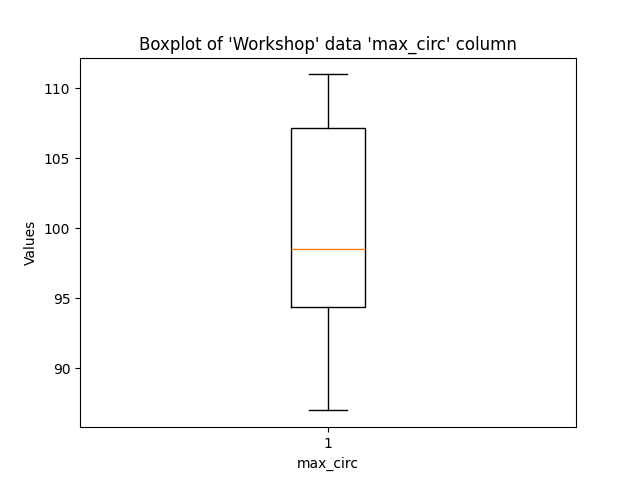
\includegraphics[width=\textwidth]{Images/Workshop_max_circ_Boxplot.png}
        \caption{}
    \end{subfigure}
    \hfill
    \begin{subfigure}[b]{0.45\textwidth}
        \centering
        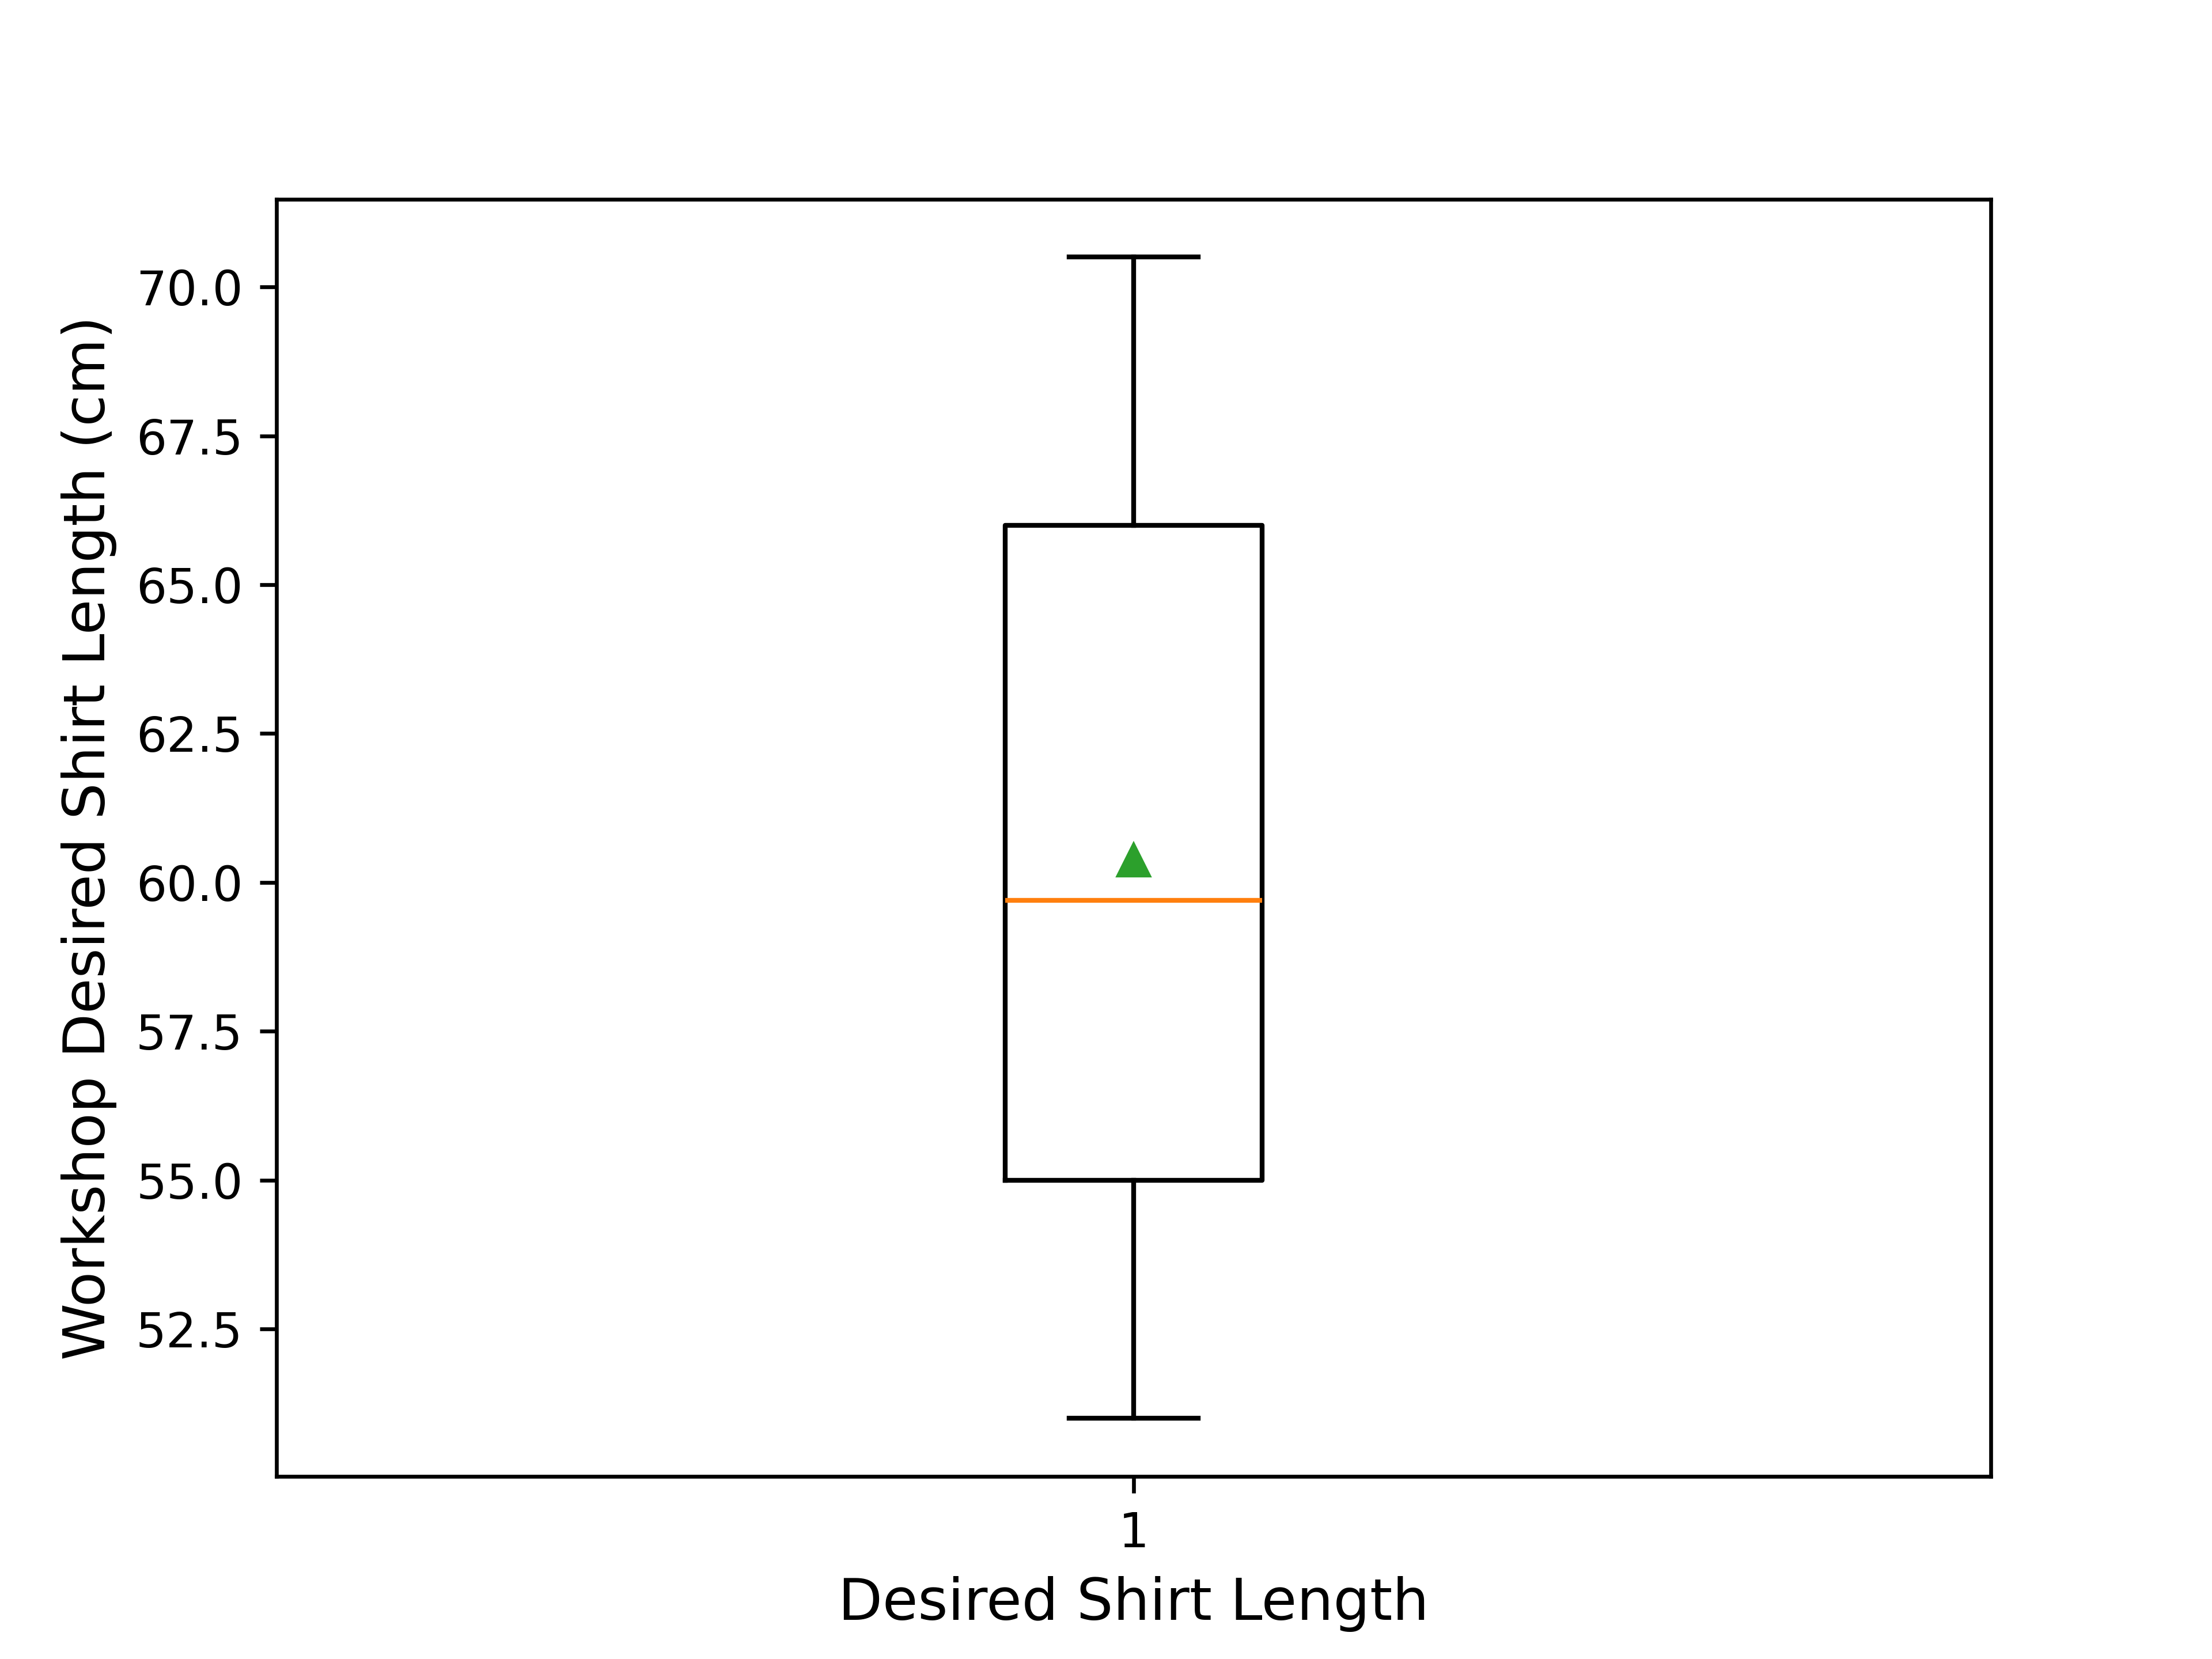
\includegraphics[width=\textwidth]{Images/Workshop_desired_shirt_length_Boxplot.png}
        \caption{}
    \end{subfigure}
    \caption{}
\end{figure}


\begin{figure} [H] % opens the figure environment. the '[H]' forces the image to be Here
    \centering % puts the image in the horizontal centre of the page
    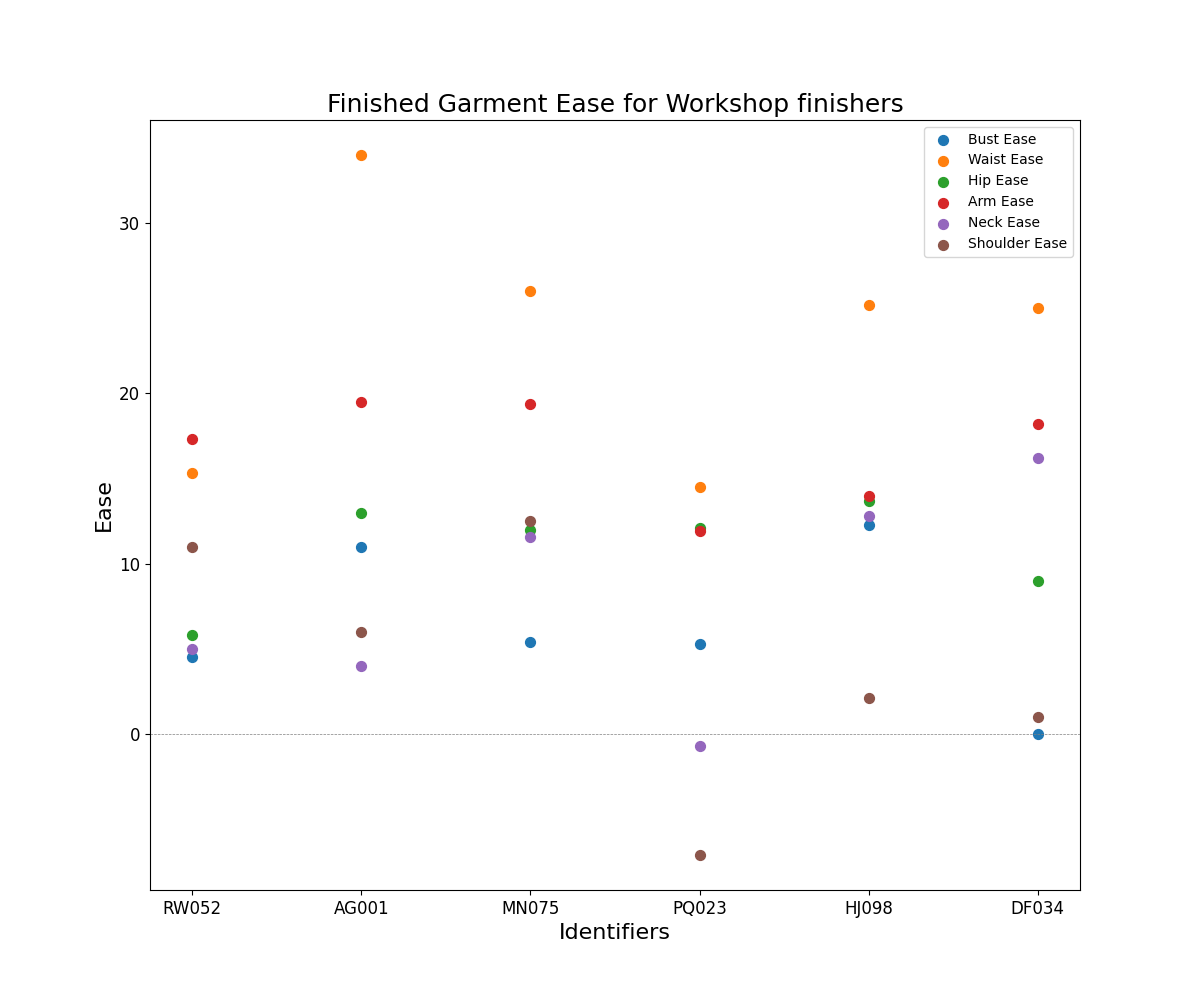
\includegraphics[width = 0.75\textwidth]{Images/FG_Ease_Plot.png} %this tells latex what graphics to include. I put my images in an 'Images' folder to aid file management, hence the Images/ before the file name. the width bit before allows you to alter the width of the image. It is also possible to use scale as well as using equations with the textwidth to make it say half the text width.
    \caption{Finished Garment eases for workshop participants}
\end{figure}

\textbf{Add likert scale plots as follows, "horizontally" per person to identify if a body type specific was not fitted well, and "vertically" per body area to identify if a body area in general was not fitted well}



\begin{figure}[H]
    \centering
    \begin{subfigure}[b]{0.45\textwidth}
        \centering
        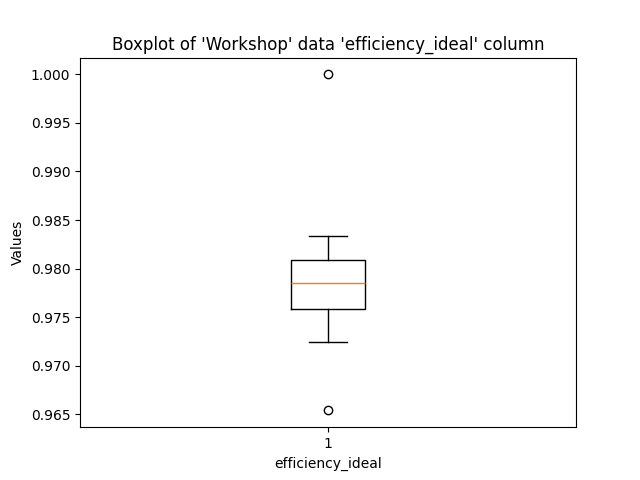
\includegraphics[width=\textwidth]{Images/Workshop_efficiency_ideal_Boxplot.png}
        \caption{}
    \end{subfigure}
    \hfill
    \begin{subfigure}[b]{0.45\textwidth}
        \centering
        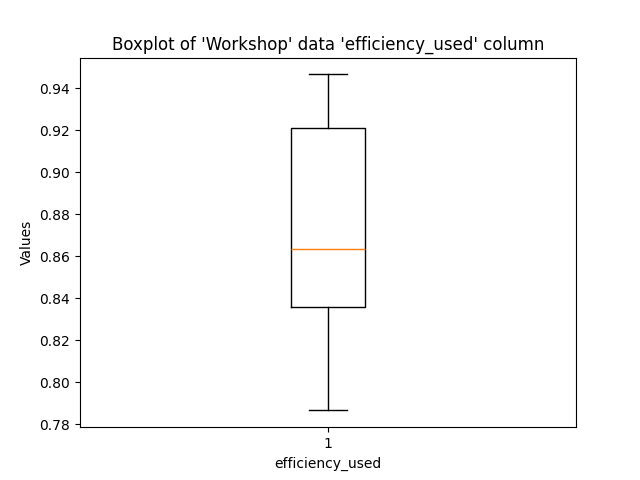
\includegraphics[width=\textwidth]{Images/Workshop_efficiency_used_Boxplot.png}
        \caption{}
    \end{subfigure}
    \caption{}
\end{figure}

\begin{figure} [H]
    \centering
    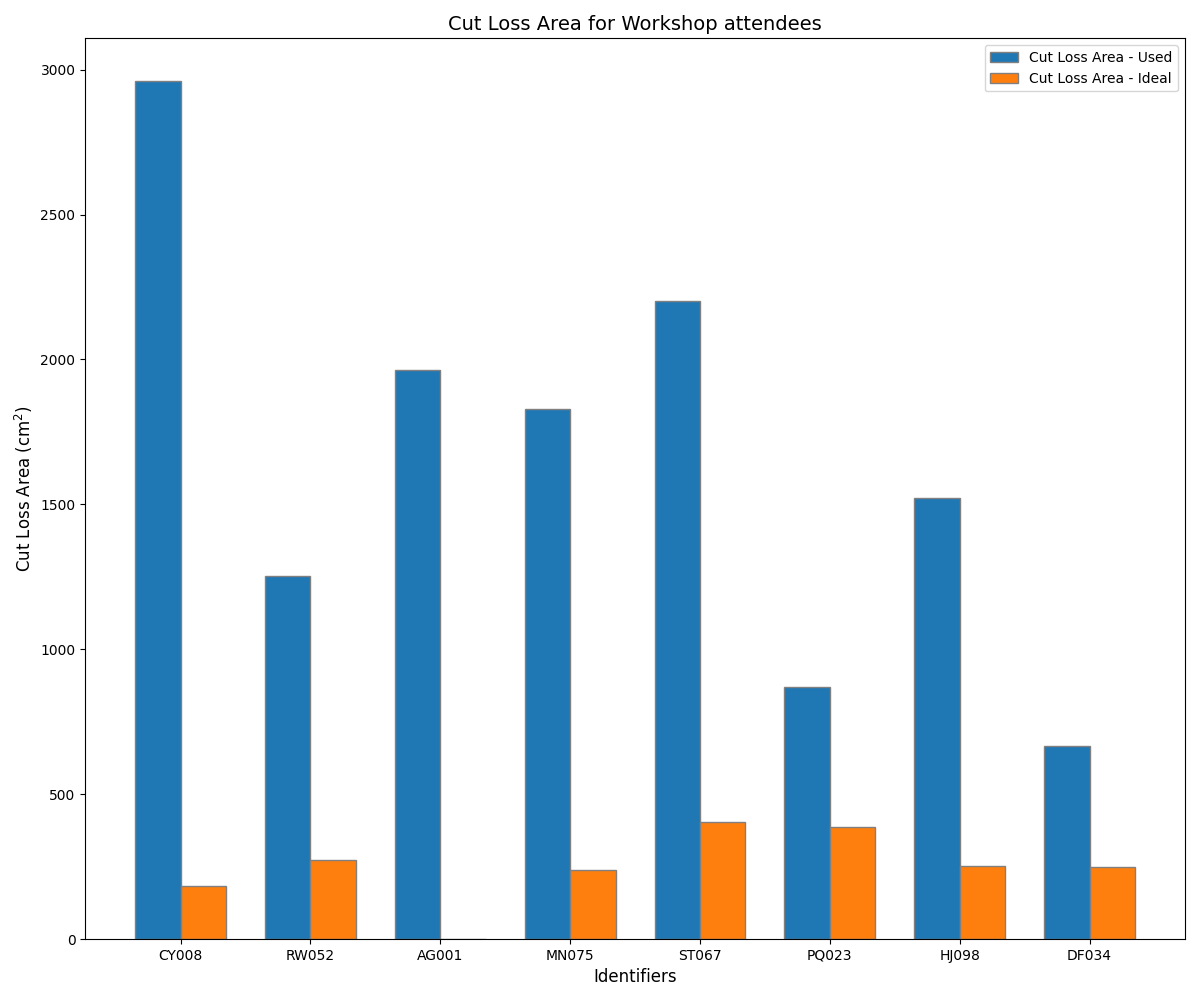
\includegraphics[width = \textwidth]{Images/Workshop_CutLossArea_Bar.png}
    \caption{Workshop Cut Loss Area}
\end{figure}
\begin{figure} [H]
    \centering
    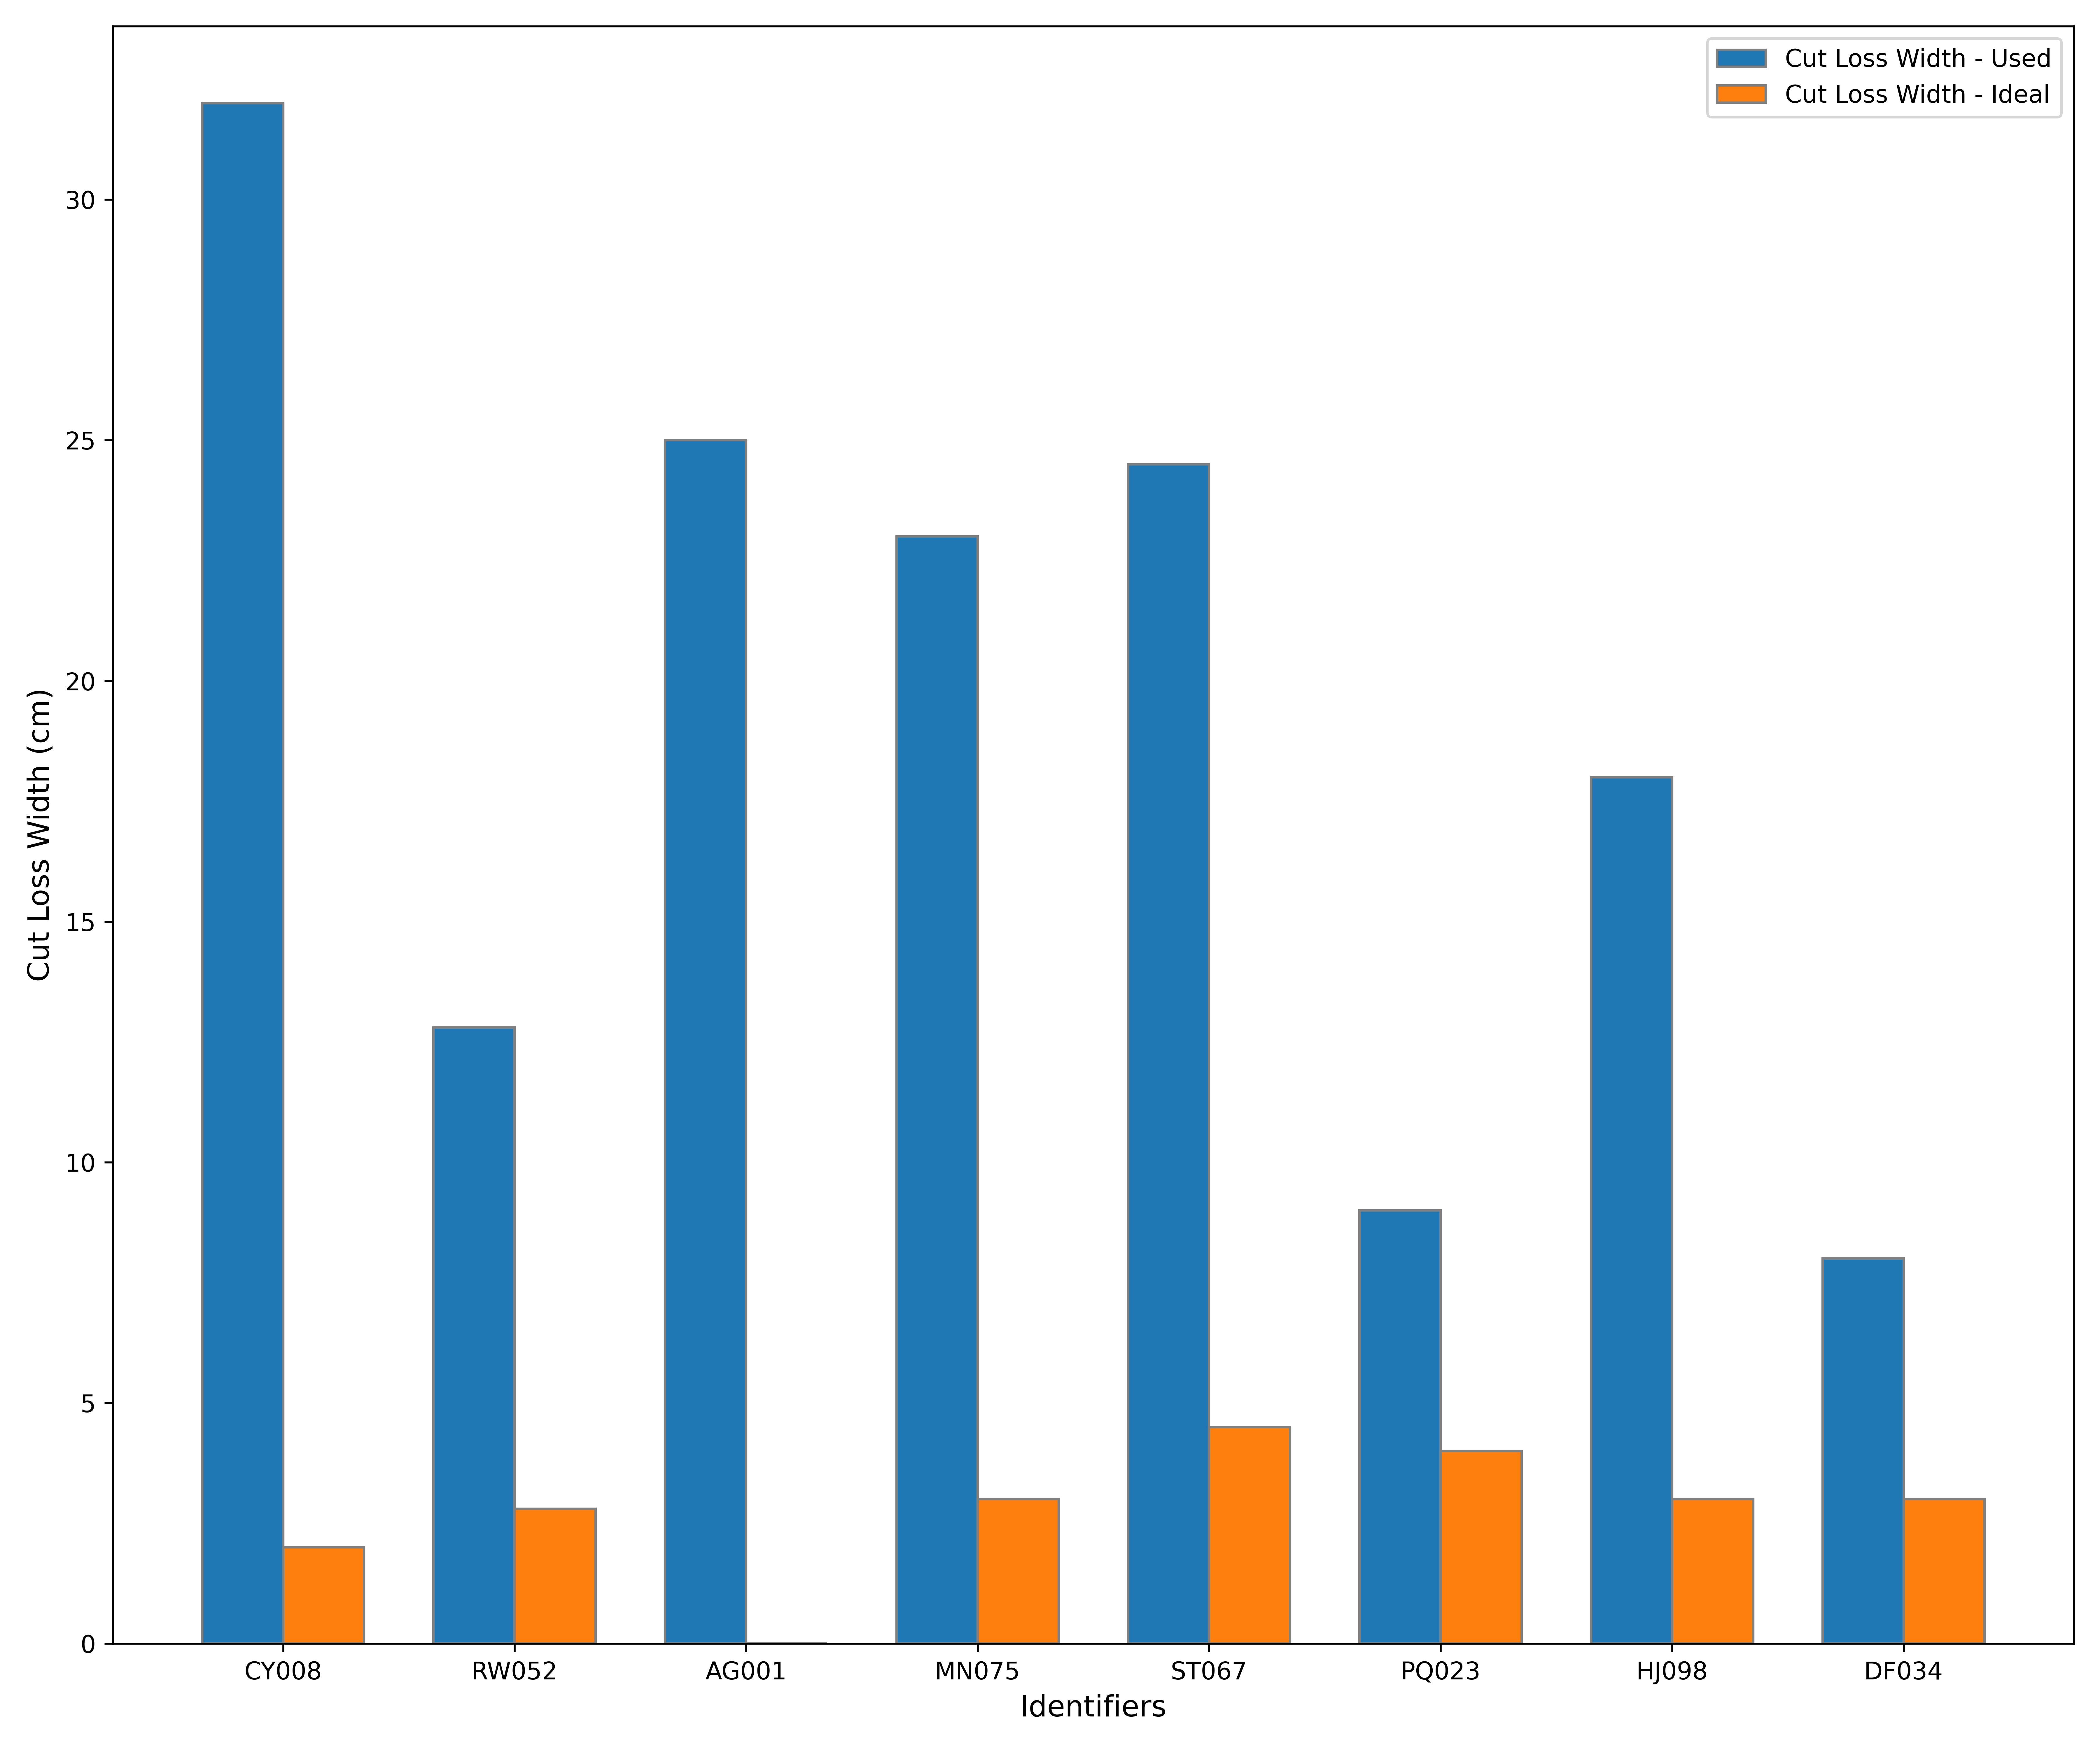
\includegraphics[width = \textwidth]{Images/Workshop_CutLossWidth_Bar.png}
    \caption{Workshop Cut Loss Width}
\end{figure}
\begin{figure} [H]
    \centering
    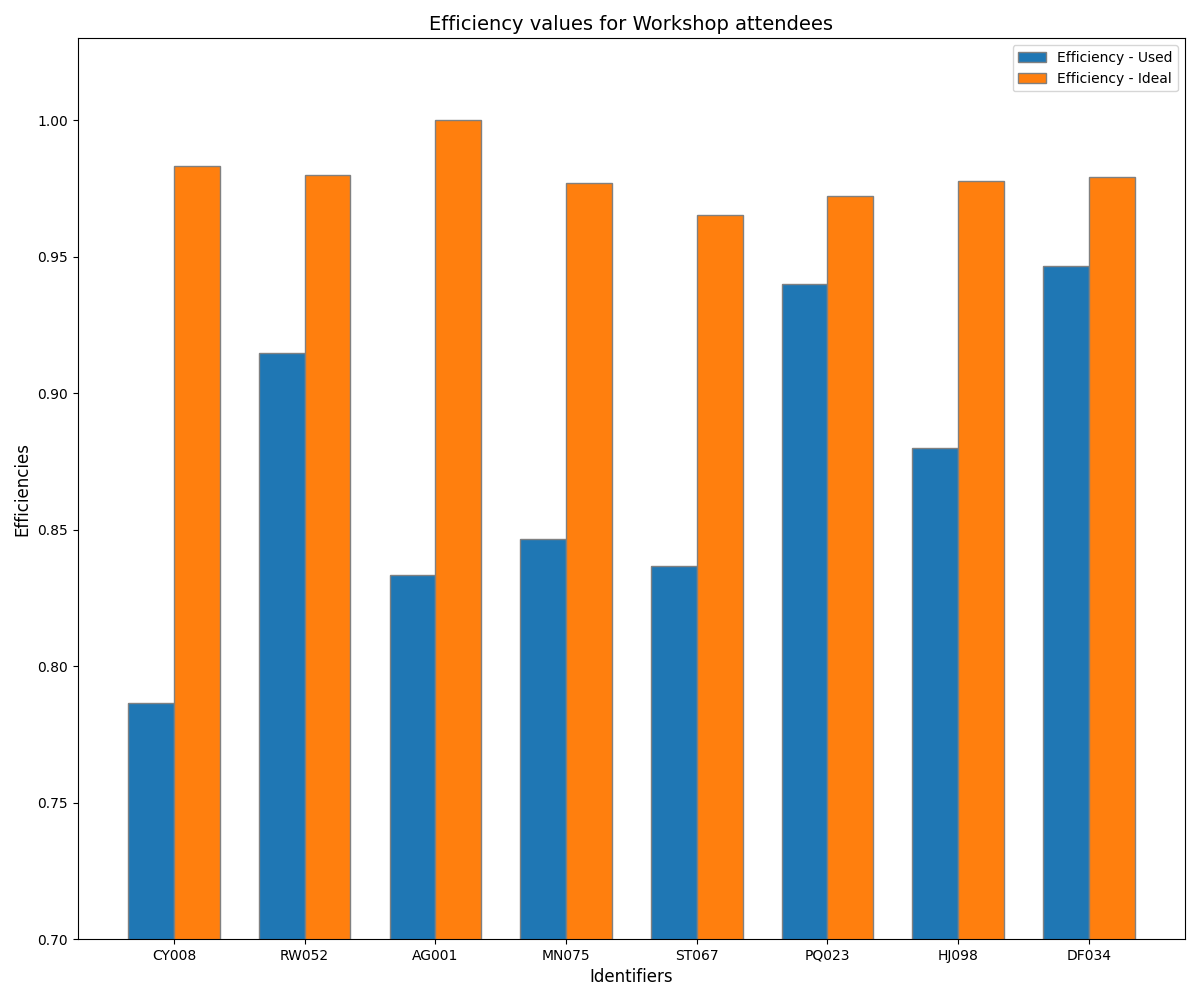
\includegraphics[width = \textwidth]{Images/Workshop_Eff_bar.png}
    \caption{Workshop Fabric Efficiency}
\end{figure}
\begin{figure} [H]
    \centering
    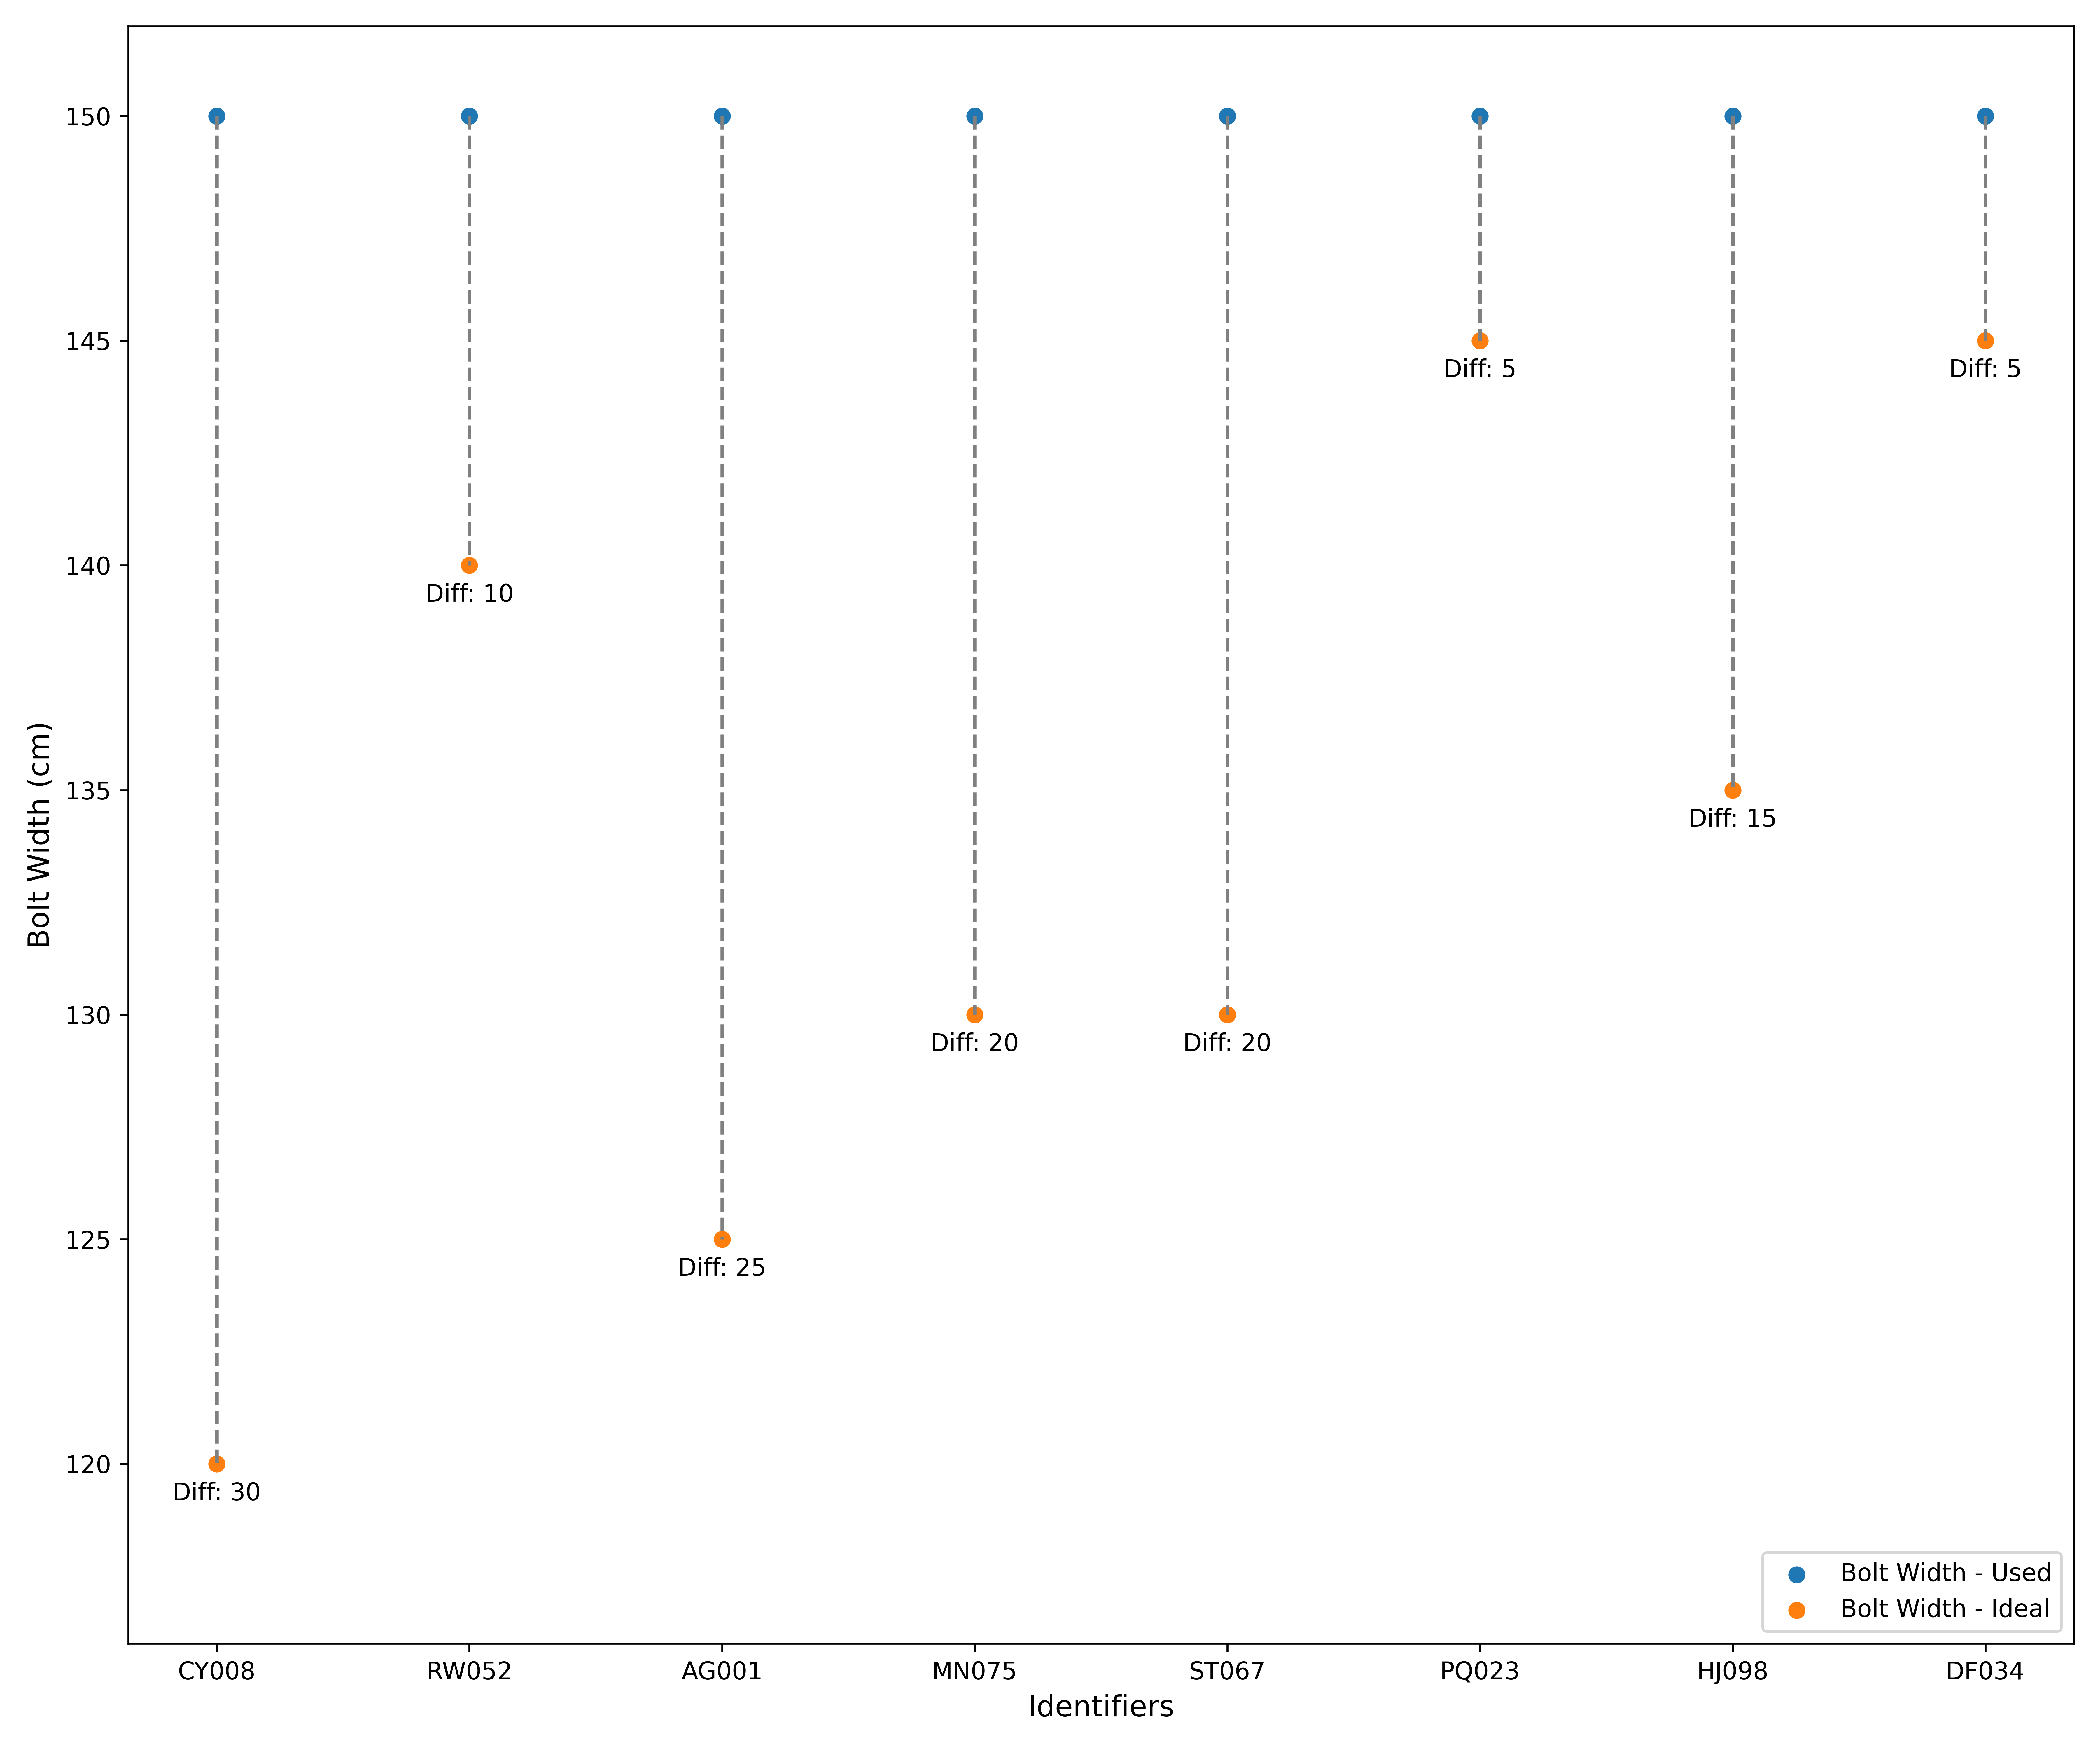
\includegraphics[width = \textwidth]{Images/Workshop_BoltWidths_Scatter.png}
    \caption{Workshop Ideal Bolts}
\end{figure}



Efficiency, bolt width, cut loss width, and cut loss area for Workshop Study comparing ideal bolt and actual used bolt.
\begin{figure} [H] % opens the figure environment. the '[H]' forces the image to be Here
    \centering % puts the image in the horizontal centre of the page
    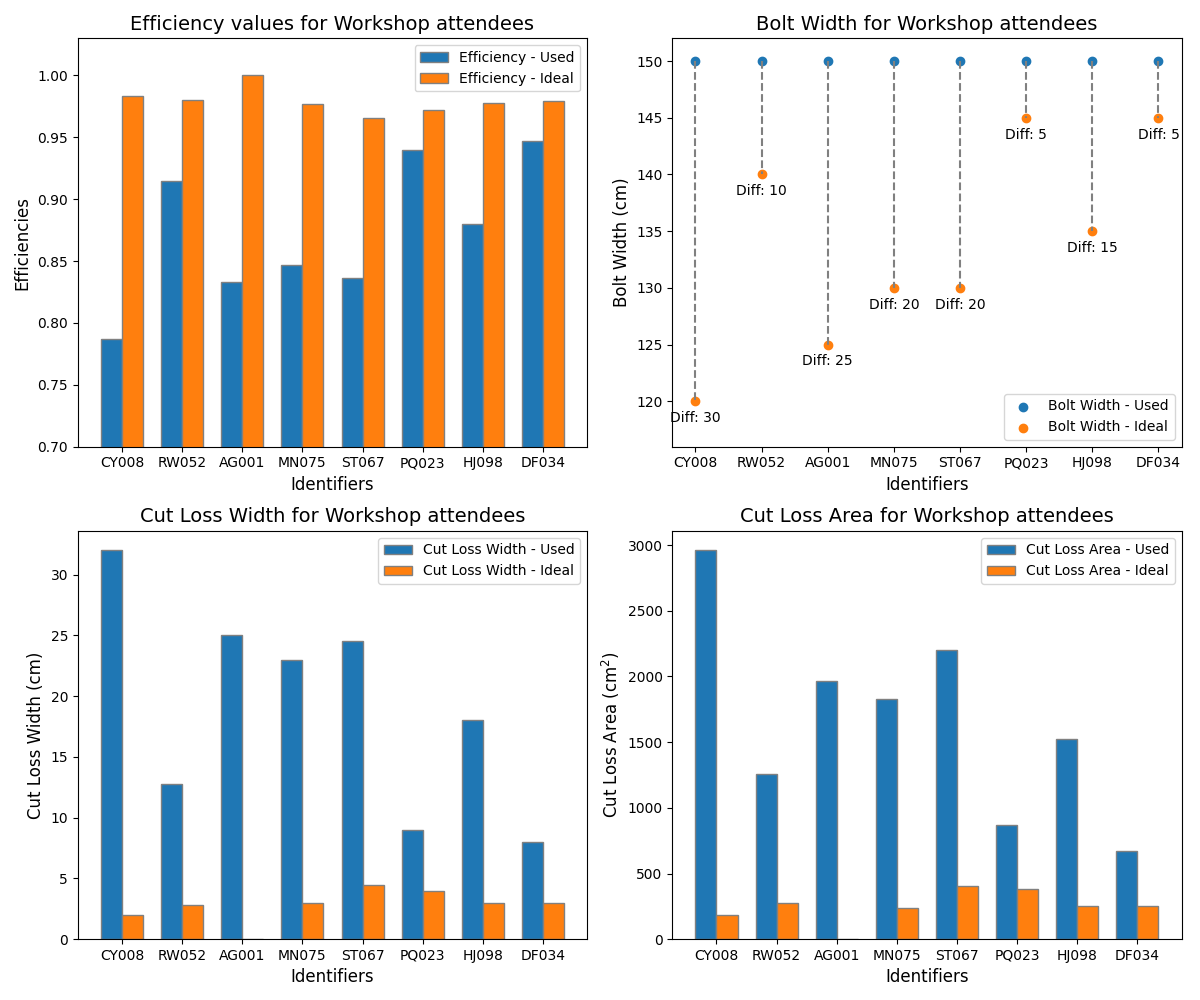
\includegraphics[width = 0.75\textwidth]{Images/Workshop_Plot.png} %this tells latex what graphics to include. I put my images in an 'Images' folder to aid file management, hence the Images/ before the file name. the width bit before allows you to alter the width of the image. It is also possible to use scale as well as using equations with the textwidth to make it say half the text width.
    \caption{Used and Ideal Efficiency Metrics for Workshop Study}
\end{figure}
All efficiencies when using ideal bolt width are greater than 95\%.







\section{Body Scans Study}
Description using max circ and shirt length

Efficiency metrics for ideal (do we still compare with 150?)
\subsection{Distibutions}
100 Scans Study persons have a mean maximum bodice circumferemce of 99.58 cm, median of 98.25 cm and a standard deviation of 8.61 cm. The mean shirt length is  cm, median of  cm, and a standard deviation of  cm.

Need to add shirt length plots
\begin{figure}[H]
    \centering
    \begin{subfigure}[b]{0.45\textwidth}
        \centering
        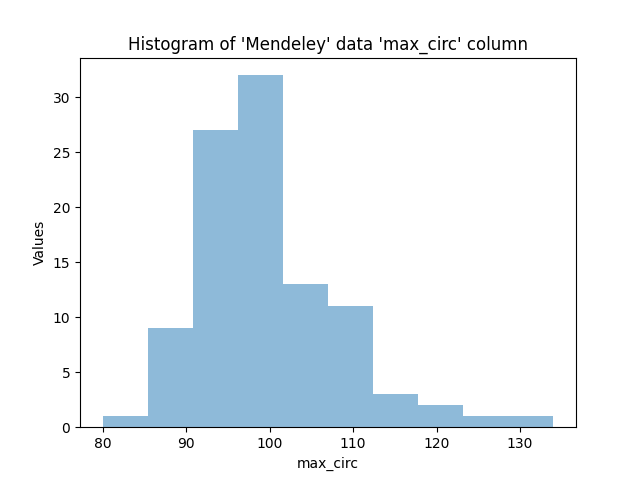
\includegraphics[width=\textwidth]{Images/Mendeley_max_circ_Hist.png}
        \caption{Histogram}
    \end{subfigure}
    \hfill
    \begin{subfigure}[b]{0.45\textwidth}
        \centering
        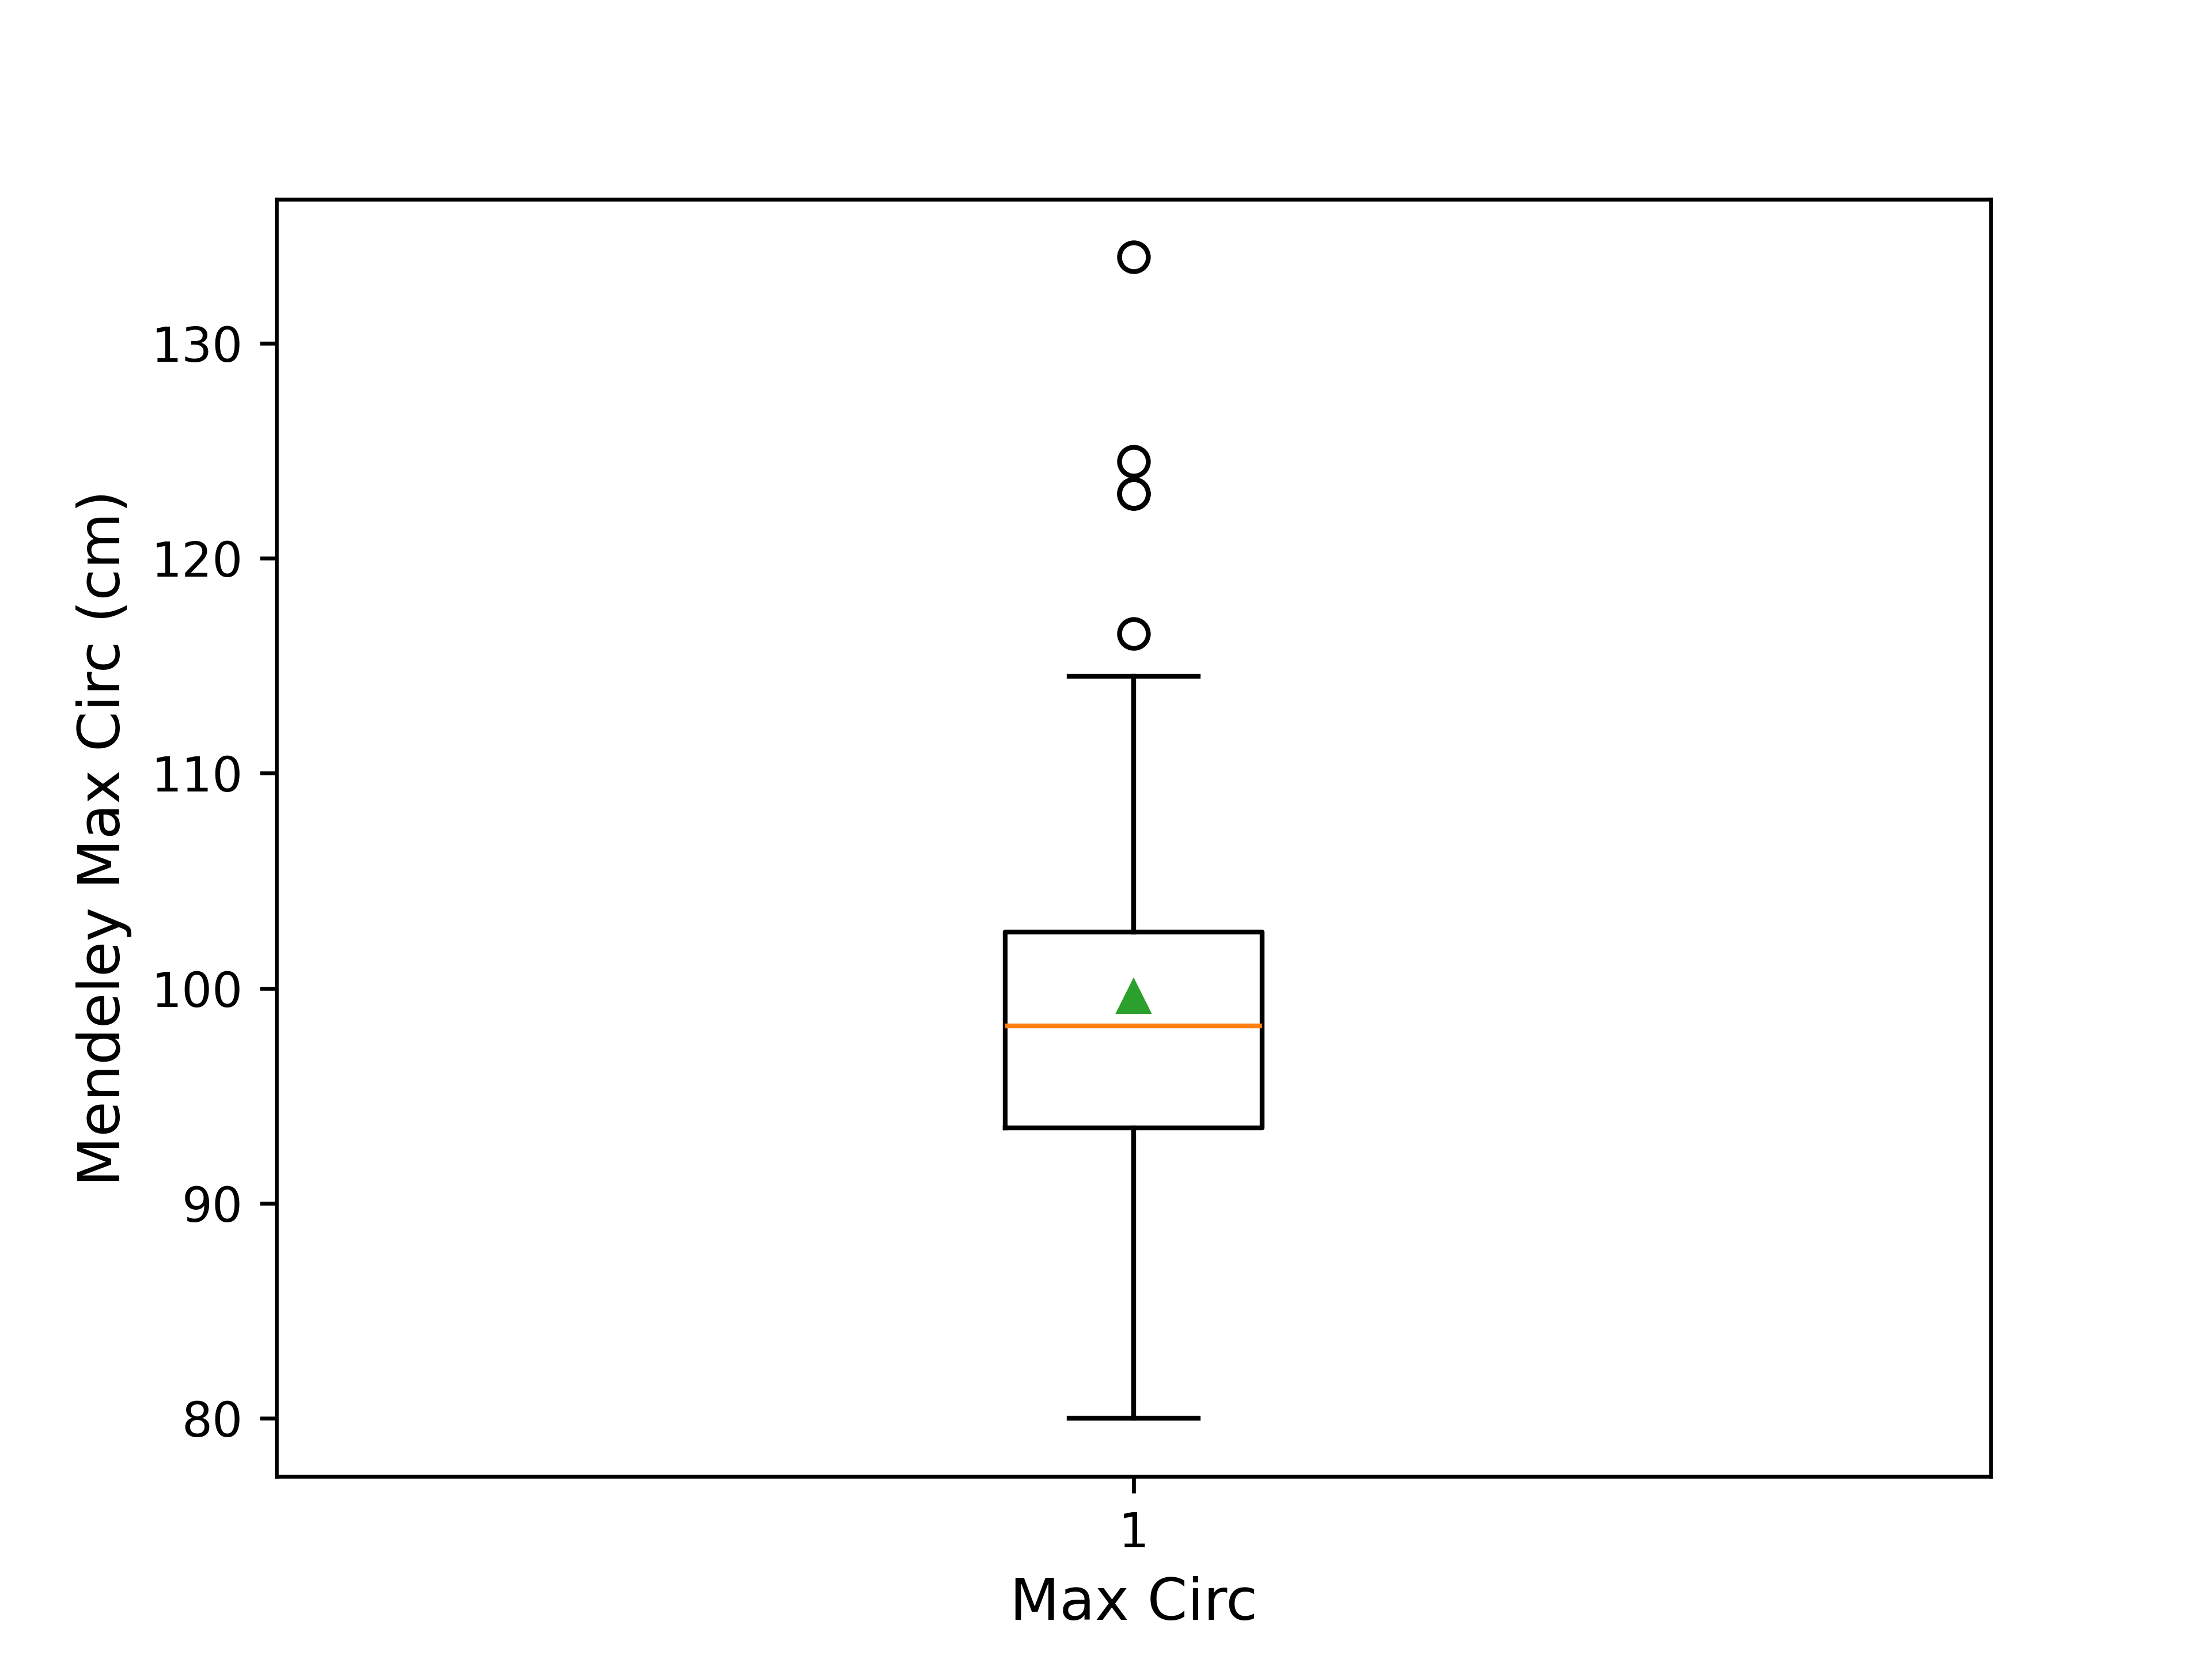
\includegraphics[width=\textwidth]{Images/Mendeley_max_circ_Boxplot.png}
        \caption{Boxplot}
    \end{subfigure}
    \caption{Distribution of max bodice circumference for 100 Scans Study}
\end{figure}

\subsubsection{Fabric Use}
Efficiency, bolt width, cut loss width, and cut loss area for 100 scans study comparing ideal bolt and hypothetical used bolt.
When using the ideal bolt width, the mean efficiency is 98\%, median efficiency is 98\%, and the standard deviation is 1\%. The mean ideal bolt width is 133 cm and median ideal bolt is 130 cm.
\begin{figure} [H] % opens the figure environment. the '[H]' forces the image to be Here
    \centering % puts the image in the horizontal centre of the page
    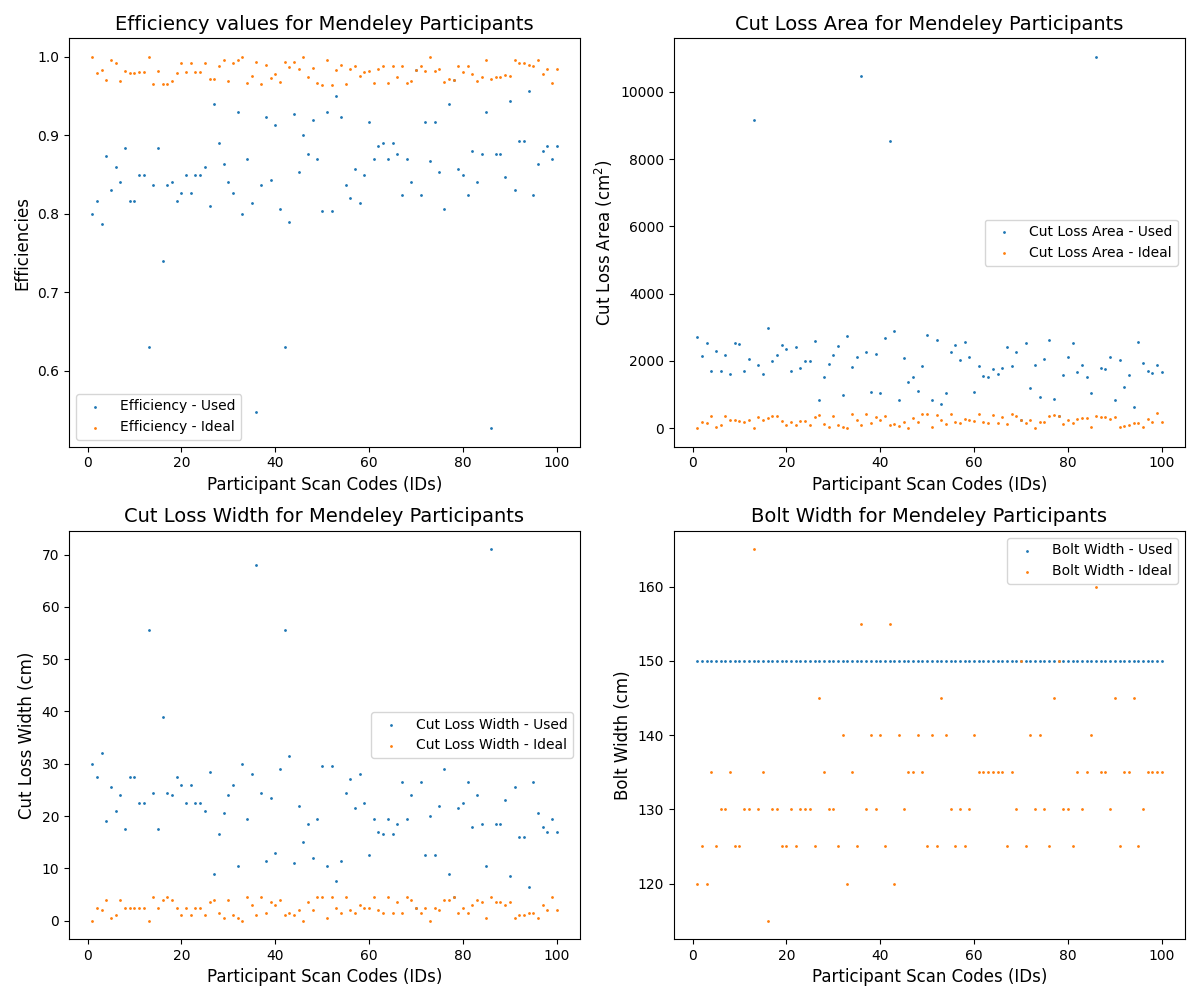
\includegraphics[width = \textwidth]{Images/Mendeley_Plot.png} %this tells latex what graphics to include. I put my images in an 'Images' folder to aid file management, hence the Images/ before the file name. the width bit before allows you to alter the width of the image. It is also possible to use scale as well as using equations with the textwidth to make it say half the text width.
    \caption{Used and Ideal Efficiency Metrics for 100 Scans Study}
\end{figure}

Cohort analysis
\begin{table} [H] % this tells the compiler that a table environment is starting
    \centering % this puts it in the horizontal centre of the page
    %\rowcolors{1}{}{Gray} % this sets up the alternating grey/white background
    \begin{tabular}{p{2cm}|p{2cm}|p{2cm}|p{2cm}|p{2cm}|p{2cm}|p{2cm}} % this sets up the tabular environment ant states the width of the columns, you could use an equation here using the \textwidth, but i have no experience with this. 
        %the following lines populate the table with data. They follow the pattern
        % item & item & item & item \\
        % where the ampersand denotes a vertical line, and the double slash, a new line.
        \textbf{Bolt Width} & \textbf{Mean Eff} & \textbf{Median Eff} & \textbf{St Dev Eff} & \textbf{Mean Loss Area} & \textbf{Median Loss Area} & \textbf{St Dev Loss Area}\\
        \hline % this produces a horizontal line, this could be used elsewhere in the table
        110& 81.7\% & 83.6\% & 6.1\% & 2620.64 & 2318.0 & 889.32\\
        115& 78.5\% & 80.0\% & 6.0\% & 3233.87 & 2922.75 & 937.46\\
        120& 76.2\% & 77.1\% & 7.4\% & 3737.44 & 3556.88 & 1207.17\\
        125& 78.7\% & 75.6\% & 12.1\% & 3526.84 & 4025.0 & 2097.15\\
        130& 83.7\% & 91.7\% & 13.5\% & 2771.99 & 934.5 & 2542.75\\
        135& 87.9\% & 92.9\% & 12.3\% & 1997.82 & 843.0 & 2501.29\\
        140& 88.8\% & 91.1\% & 9.2\% & 1716.44 & 1131.0 & 2025.64\\
        145& 87.3\% & 88.1\% & 8.1\% & 1865.09 & 1491.63 & 1849.15\\
        150& 85.2\% & 85.5\% & 7.1\% & 2158.84 & 1890.75 & 1679.22\\
        155& 83.3\% & 83.1\% & 6.2\% & 2418.42 & 2333.63 & 1388.62\\
        160& 81.2\% & 80.6\% & 5.4\% & 2752.84 & 2795.13 & 1076.74\\
        165& 79.1\% & 78.3\% & 5.2\% & 3089.52 & 3250.13 & 782.20\\
        \end{tabular}
    \caption{Description of Cohort Analysis on Different Bolts for 100 Scans Study}
\end{table}
\textbf{SHOULD CHANGE FORMAT OF GRAPHS BELOW BECAUSE NOT CONTINOUS???}
\begin{figure}[H]
    \centering
    \begin{subfigure}[b]{0.45\textwidth}
        \centering
        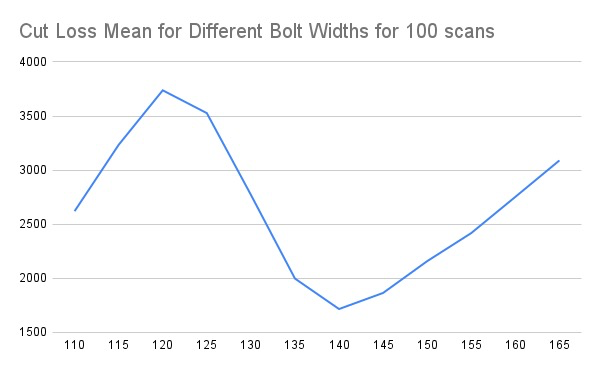
\includegraphics[width=\textwidth]{Images/Cut Loss Mean for Different Bolt Widths for 100 scans.png}
        \caption{Cut Loss Area}
    \end{subfigure}
    \hfill
    \begin{subfigure}[b]{0.45\textwidth}
        \centering
        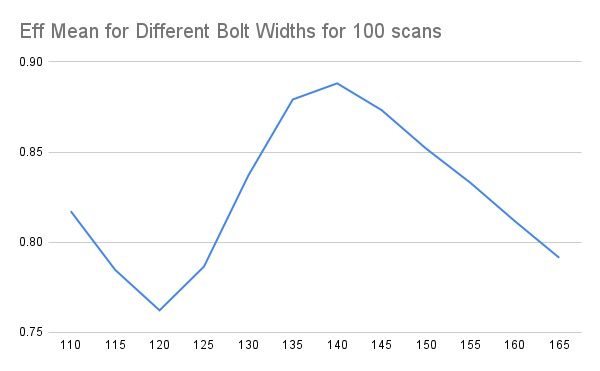
\includegraphics[width=\textwidth]{Images/Eff Mean for Different Bolt Widths for 100 scans.png}
        \caption{Efficiency}
    \end{subfigure}
    \caption{Mean Cut Loss Area Used and Efficiency Used for Different Bolt Widths for 100 Scans Study}
\end{figure}

For this cohort, using a 140 cm wide fabric bolt minimises the cut loss area and maximises the efficiency.

Count of pattern orientation on starting fabric and possibility of embellishment potential for various bolt widths ranging from 110 to 160 cm.
\begin{figure} [H] % opens the figure environment. the '[H]' forces the image to be Here
    \centering % puts the image in the horizontal centre of the page
    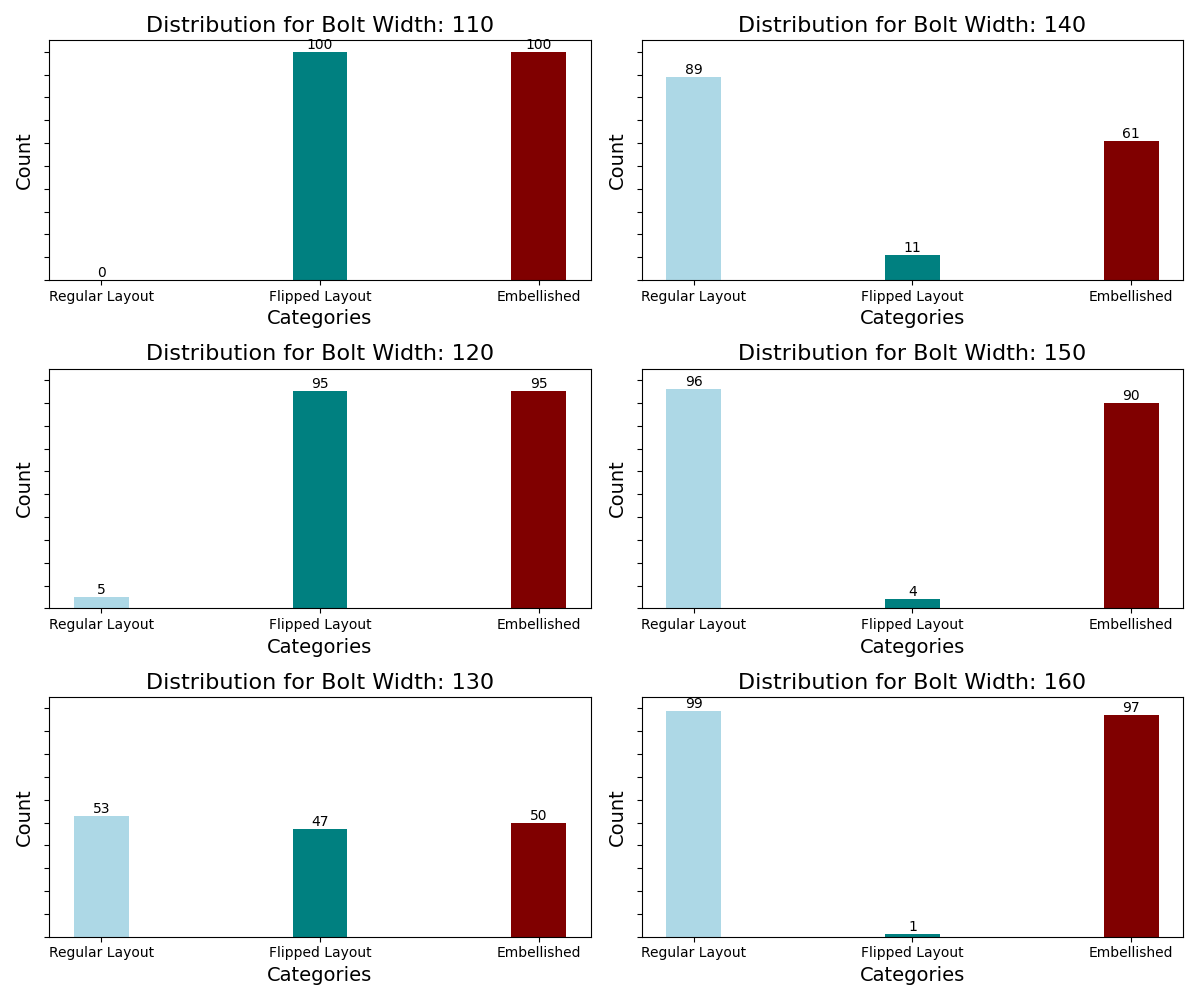
\includegraphics[width = \textwidth]{Images/Mendeley_Bar.png} %this tells latex what graphics to include. I put my images in an 'Images' folder to aid file management, hence the Images/ before the file name. the width bit before allows you to alter the width of the image. It is also possible to use scale as well as using equations with the textwidth to make it say half the text width.
    \caption{Layout and Embellishment Possibility for 100 Scans Study}
\end{figure}
For the range of bolt widths between 110 and 160 cm, each pattern generated for the Mendeley dataset participants will fit in the regular or rotated orientation. No mitigation strategies need to be employed within this range of bolts.

\textbf{ADD recoup of cut loss area due to embellishment}

\section{Personal Case Study}
